% What Context Compression Cannot Buy
% Version 2 -- 2026-09-23 (v1: 2026-09-22, doi:10.5281/zenodo.22897854)
% pdflatex + bibtex + pdflatex x2. Standard packages only.
\documentclass[11pt]{article}
\usepackage[margin=1in]{geometry}
\usepackage{booktabs}
\usepackage{amsmath}
\usepackage{graphicx}
\usepackage{hyperref}
\usepackage{xcolor}
% Latin Modern is scalable; microtype's font expansion refuses to run on the
% default bitmap CM fonts.
\usepackage{lmodern}
\usepackage[T1]{fontenc}
\usepackage{microtype}
% \citet / \citep and the plainnat style both come from natbib; loaded before
% hyperref so the citation links are built correctly.
\usepackage{natbib}

\hypersetup{colorlinks=true, linkcolor=blue!50!black, citecolor=blue!50!black,
            urlcolor=blue!50!black}

% Draft markers -- every one of these must be gone before submission.
\newcommand{\TODO}[1]{\textcolor{red}{\textbf{[TODO: #1]}}}
\newcommand{\CHECK}[1]{\textcolor{orange}{[verify: #1]}}

\title{What Context Compression Cannot Buy:\\
       Diagnosing the Recall Ceiling with a Frozen Backbone}

\author{Xin Gao\\
  \texttt{hoshi@stu.xaut.edu.cn}}

\date{Version 2, 23 September 2026}

\begin{document}
\maketitle

\begin{abstract}
Compression of a transformer's KV cache is usually reported as one number: the
fraction of full-context quality retained. We ask what the missing fraction is
made of. Training only 3.67M memory-slot parameters with the backbone frozen,
we find that fraction is set by a single property of the task---how much of the
answer can be copied from the context rather than inferred.

Splitting predicted tokens on that property separates them sharply: tokens that
never appeared recover at $+202\%$, above the verbatim cache they replace, while
tokens seen exactly once reach $+45\%$. Posed as a task---recover a random
five-digit code hidden in the context---64 learned slots answer none of 150
trials and leave the model worse off than with no context at all, while 84
verbatim entries answer $98\%$ when they are the right ones.

The same property says where each kind of memory pays. On held-out text, 64
learned slots are worth as much as 576 entries selected by H2O, and giving 64 of
H2O's 576 entries to the slots recovers $101\%$ of the gap, more than the full
cache. On the needle task the slots are dead weight and everything rests on
selection: SnapKV with the question in its window answers $99\%$, the same
policies committing before the question arrives answer at most $20\%$, and our
own retrieval, one set of positions shared by every layer, answers $12\%$.
Across 0.6B to 14B each resource alone is flat, while what the slots add behind
a fixed selection peaks at 1.7B--4B and halves by 14B.

We also quantify two measurement hazards: fine-tuning the backbone improves the
no-context baseline by 0.58 nats, inflating every relative compression metric,
and pooling scale points measured under different quantisation and corpora
manufactured a clean monotone trend that a controlled sweep does not show.
This version corrects a bug in version 1's attention scoring and every
conclusion that rested on it.
\end{abstract}

\section{Introduction}

Work on shrinking the KV cache of a long-context transformer---by eviction, by
low-rank or low-bit approximation, by learned summarisation into a fixed budget
of slots---reports its result as a retention figure: this method keeps $x\%$ of
full-context quality at $y\times$ compression. The figure is useful for choosing
a method. It says nothing about the $1-x$.

This paper is about the $1-x$. We do not propose a compression method; several
of the components we use were introduced elsewhere and we cite them as such
(\S\ref{sec:related}). We use a deliberately minimal setup---a frozen backbone
with a few million trainable memory-slot parameters---as an instrument, and ask
two questions about where compressed context loses to verbatim context.

\paragraph{Contribution 1: the ceiling is made of precise recall
(\S\ref{sec:copyability}).}
We group the tokens being predicted by whether that token appeared anywhere in
the preceding context, i.e.\ by whether the answer was available to copy
(Table~\ref{tab:copyability}). The
groups behave qualitatively differently rather than by degree. On tokens that
never appeared, a 64-slot learned state recovers $+202\%$ of the gap between no
context and full context---it is more useful than the verbatim cache it replaces,
because it was optimised to predict the continuation whereas raw KV was not. On
tokens that appeared exactly once, the same state recovers $+45\%$. Since the
copyable group is $79.6\%$ of the suffix and carries $76.0\%$ of the gap, the
ceiling on abstractive compression is a property of the task, not a deficiency
of the compressor. We then state the same claim as a retrieval task
(\S\ref{sec:needle}), where the answer is a random code and abstraction is not
merely insufficient but actively harmful. The same axis predicts where each
kind of memory pays (\S\ref{sec:baselines}): on natural text the learned state
adds a fixed-budget gain behind any selector, including the strongest
training-free one we ran, while on the needle task it is dead weight and the
outcome rests on whether the selector sees the question and may choose per
attention head. To our knowledge this decomposition has not been reported for
compressed context; the nearest work stratifies tokens by $n$-gram novelty in
\emph{uncompressed} long-context models \citep{tokensbenefit}, or contrasts
topical against unexpected needles at the task level \citep{gistboundary}.

\paragraph{Contribution 2: retrieval and compression are separable and roughly
equal, and only the state's marginal value responds to scale
(\S\ref{sec:decomposition}, \S\ref{para:scale}).}
Pairing the abstract state with a small set of exactly-retrieved verbatim KV
entries is a natural architecture and has been proposed before
\citep{strongdrafts,specache}. What has not been measured, to our knowledge, is
the attribution: we fix the retrieved entries and swap only the state behind
them (absent / trained / randomly initialised), and independently fix the state
and swap only the anchor \emph{source} (a deployable query against an
answer-aware oracle). This closes a $2\times2$ design in which each factor's
contribution can be read holding the other fixed, and the result survives
replacing our retrieval with a stronger training-free selector
(\S\ref{sec:baselines}). Agent-memory systems have
compared ``read the summary'' against ``fetch the source''
\citep{justmem,infinimemory}, but with both the retrieval set and the summariser
varying together. The scale axis separates them a second time: across five
backbone sizes each resource is flat on its own, while what the learned state
adds behind a fixed selection peaks at 1.7B--4B and roughly halves by 14B, behind
three different selectors (\S\ref{para:scale}). A single-resource account does
not predict that.

\paragraph{Contribution 3 (a caveat, not a claim): two measurement hazards
(\S\ref{sec:hazards}).}
Relative compression metrics normalise by the distance between a no-context
lower bound and a full-context upper bound. If the backbone is fine-tuned during
compression training, the lower bound moves: we measure $0.58$ nats of
improvement on ``predict the continuation with no context at all,'' shrinking the
denominator by a third and inflating recovery from $+8\%$ to $+66\%$ on the
identical configuration. This is not a new observation so much as a
quantification of one: \citet{ccm} report the same phenomenon as a training
pathology (the model learns to answer without consulting its memory) and freeze
the LM in response, and \citet{simplecc} adopt an almost identical normalisation
to control for questions answerable without context. Our contribution is to
frame it as an \emph{evaluation} confound with a measured magnitude, and to note
the boundary: it affects relative metrics only, not absolute task accuracy.
Second, we report seed variance, which is rarely reported in this literature and
is largest exactly where it matters most. We also give two worked examples of
what skipping this costs, both from our own earlier drafts of the scale
comparison: mismatched prediction lengths put the gap at 0.492 against 0.822
nats and made the recovery figures incomparable, and pooling points measured
under different quantisation and corpora produced a clean monotone trend that
the controlled sweep does not show (\S\ref{para:scale}).

\section{Setup}
\label{sec:setup}

\paragraph{Compressor.}
A context window of $n$ tokens is consumed in segments. Each segment is encoded
with the frozen backbone and reduced to $k$ learned memory slots, which are
prepended to the next segment's attention as synthetic KV entries. The only
trainable parameters are the slot embeddings ($0.03$M) and, in the \emph{deep}
variant, a per-layer additive bias applied at memory positions only
($3.67$M, in the manner of prefix tuning \citep{ptuningv2}). Because attention is
causal and the bias is restricted to memory positions, the backbone's behaviour
on real tokens is bit-identical to the unmodified model.

\paragraph{Metric.}
For a held-out suffix we measure mean token cross-entropy under three
conditions: \textsc{upper} (the full verbatim KV cache of all $n$ preceding
tokens), \textsc{lower} (no context at all), and the condition under test. We
report
\begin{equation}
\text{recovery} = \frac{\textsc{lower} - \text{test}}{\textsc{lower} - \textsc{upper}},
\label{eq:recovery}
\end{equation}
in nats. $1.0$ means indistinguishable from the full cache and $0$ means the
context was worthless. \textbf{Values above $1.0$ are attainable and are not an
error}: the learned slots are trained to predict the next segment, whereas the
verbatim cache is simply what the model happened to write down, so a compressed
state can be more useful than the text it summarises. We call
$\textsc{lower}-\textsc{upper}$ the \emph{gap}, and note that it is a property of
the corpus rather than of the method: it is $1.269$ nats on real dialogue and
$0.286$ nats on Project Gutenberg prose, meaning long context is worth little on
coherent narrative to begin with (\S\ref{sec:limitations}).

\paragraph{Anchors.}
In the hybrid conditions, a budget of $a$ verbatim KV entries (``anchors'') is
selected from the offloaded full cache and paged back in alongside the $k$ slots.
Selection policies are compared in \S\ref{sec:decomposition}. Two details are
load-bearing and easy to get wrong. First, any scheme that retains only part of
the cache must pin the first few positions as an \emph{attention sink}
\citep{streamingllm}; without it recovery collapses to $-400\%$. Second,
positions must accumulate across segments rather than restart, which is worth
4 points.

\paragraph{Scale and cost.}
Qwen3-0.6B \citep{qwen3} for every measurement, with the hybrid architecture
checked against 1.7B (\S\ref{sec:levers}); windows of 4096 tokens in
\S\ref{sec:copyability} and 8192 in \S\ref{sec:decomposition}, stated per table
because the two are not comparable. Everything ran on a single RTX 4060 Laptop
(8\,GB); training one memory module takes roughly 12 minutes, and no cloud
compute was used for any number in this paper.

\section{The ceiling is made of precise recall}
\label{sec:copyability}

Two levers that should raise a compressor's ceiling do not
(\S\ref{sec:levers}): more training and more slots. At a fixed backbone, then,
the residual is not something the compressor is failing to try hard enough at.
The candidate is precise recall---the identifier introduced 2000 tokens ago, the
number, the proper noun. Verbatim KV can be copied from. A summary cannot
reconstruct a string it did not store. Scale does move the level
(\S\ref{para:scale}), and we return at the end of this section to what it does
and does not change.

We test this by partitioning the predicted suffix. For each target token we ask
whether that token appears anywhere in the preceding context, and compute
per-token cross-entropy within each group under all three conditions. Only the
abstract state is provided---no anchors---so the comparison isolates what
abstraction alone can serve.

\begin{table}[ht]
\centering
\small
\begin{tabular}{lrrrrr}
\toprule
target token & share & \textsc{lower} & \textsc{upper} & gap (nats) & recovery \\
\midrule
never appeared      & 20.4\% & 5.731 & 5.518 & $\mathbf{0.213}$ & $+202\%$ \\
appeared            & 79.6\% & 3.542 & 2.401 & $\mathbf{1.141}$ & $+58\%$ \\
\quad exactly once  &  9.6\% & 5.190 & 4.014 & 1.176 & $+45\%$ \\
\quad 2--5 times    & 19.4\% & 4.539 & 3.045 & 1.494 & $+48\%$ \\
\quad 6+ times      & 50.6\% & 2.848 & 1.849 & 0.999 & $+67\%$ \\
\midrule
all                 & 100\%  & 3.989 & 3.038 & 0.951 & $+65\%$ \\
\bottomrule
\end{tabular}
\caption{Cross-entropy by token copyability, abstract state only (64 slots,
8 hops over 4096 tokens), mean of three independently trained modules.
\textsc{lower} is no context, \textsc{upper} the full verbatim cache. Seed
spread is 3.0--4.3 points on the large groups but 9.1 on ``exactly once''
($n{=}1176$) and 11.3 on ``never appeared'', where the small gap in the
denominator amplifies it---see the caution below.}
\label{tab:copyability}
\end{table}

\paragraph{Read the gap column first.}
The cleanest statement here does not involve our metric at all. Having the entire
verbatim context is worth $1.141$ nats on tokens that appeared in it and $0.213$
nats on tokens that did not. Long context earns most of its value on material
that can be copied: the copyable group is $79.6\%$ of the suffix and carries
$76.0\%$ of the total gap, a figure identical across all three seeds because it
depends only on the corpus and not on the module. Whatever a compressor does,
this is the shape of what it is compressing.

\paragraph{Recovery, with a caution about the denominator.}
On tokens that never appeared, the 64-slot state recovers $+202\%$---substantially
more useful than the verbatim cache it replaces, because it was trained to
predict the continuation whereas the cache is merely what the model wrote down.
On tokens that appeared exactly once it recovers $+45\%$, and recovery rises
monotonically with how often the token was seen ($+45 \to +48 \to +67$). The
caution: those extreme groups also carry the largest seed spread, and not by
accident. Recovery divides by the gap; the never-appeared gap is $0.213$ nats;
dividing by a small number magnifies everything, including noise. The ordering is
robust---$+202$ against $+58$ is a separation of 144 points against spreads of 11
and 4---but the value $202$ itself is not stable to three significant figures,
and we would not report it without the gap column beside it. This is a general
hazard when a relative compression metric is evaluated on subsets, and a reason
to prefer absolute nats when slicing.

\paragraph{The ordering is a property of the task; the levels are not.}
Repeating the split at 0.6B and 4B separates what is fixed from what is not.

\begin{table}[ht]
\centering
\small
\begin{tabular}{lrrrrr}
\toprule
 & once & 2--5 & 6+ & never & all \\
\midrule
0.6B & $+30.9$ & $+40.1$ & $+60.1$ & $+126.7$ & $+53.6$ \\
4B   & $+56.6$ & $+56.7$ & $+71.0$ & $+165.2$ & $+72.7$ \\
\midrule
change & $\mathbf{+25.7}$ & $+16.6$ & $\mathbf{+10.9}$ & $+38.5$ & $+19.1$ \\
\bottomrule
\end{tabular}
\caption{The same partition at two scales, single seed each. Two mismatches make
the absolute values here lower than Table~\ref{tab:copyability} and not
comparable to it: these modules were trained at the shorter prediction length
and evaluated over a full segment, and the 4B backbone is NF4-quantised while
0.6B is bf16. Only the pattern across columns should be read. 1.7B is omitted
because that particular checkpoint diverged under recursion
(\S\ref{sec:limitations}).}
\label{tab:copyscale}
\end{table}

Which tokens are hard does not change---the ordering holds at both scales, and
tokens seen once remain the worst-served group by a wide margin. How hard they
are does change, and in the direction we did not predict: the hardest column
improves most ($+25.7$) and the easiest improves least ($+10.9$). So the ceiling
is not a fixed property of abstractive compression. It is a property of what a
\emph{given} backbone can compress, and a larger one recovers a substantial part
of what the smaller one loses on precisely the tokens we called incompressible.
We therefore state the finding as the ordering rather than the level, and note
that an extrapolation to ``a large enough model would not need exact recall at
all'' is not supported by two points.

\paragraph{What follows.}
Two readings. First, abstraction is not a degraded copy of verbatim context but a
different thing---better on some tokens, much worse on others. Aggregate recovery
figures approaching $100\%$ should therefore not be read as ``nearly as good as
having the text,'' since they average over groups that behave in opposite
directions. Second, the practical one: at a fixed backbone the residual lives in
copyable tokens, and the way to buy it back is not a larger abstraction
budget---\S\ref{sec:levers} shows doubling it buys $0.6$ points---but a small
number of \emph{exact} entries. \S\ref{sec:decomposition} measures what that
buys.

\subsection{The same claim, stated as a task}
\label{sec:needle}

Everything above is perplexity on held-out text, which is the form of evidence a
reader has least reason to trust. The claim it supports---that what compression
cannot buy is precise recall---can be stated as a task instead. We hide a
uniformly random five-digit code in the context (``the secret code for
warehouse 7 is 48213''), place the question at the end, and ask for the digits
back. Copyability here is total rather than statistical: the code is drawn at
generation time, so no prior over language helps, and a memory that did not
store the digits cannot produce them.

\begin{table}[ht]
\centering
\small
\begin{tabular}{lrrr}
\toprule
memory available at question time & entries & recovery & exact match \\
\midrule
full verbatim cache                        & 4096 & $+100\%$  & $\mathbf{100\%}$ \\
no context                                 & 0    & $0\%$     & $0\%$ \\
\midrule
abstract slots                             & 64   & $\mathbf{-28.6\%}$ & $\mathbf{0\%}$ \\
anchors retrieved by the question          & 512  & $+14.0\%$ & $13\%$ \\
\quad the same $+$ 64 slots                & 576  & $+13.2\%$ & $12\%$ \\
SnapKV, question in its window             & 576  & $+99.6\%$ & $\mathbf{99\%}$ \\
oracle: the needle itself $+$ sink $+$ 64 slots & 84 & $+94.4\%$ & $98\%$ \\
\bottomrule
\end{tabular}
\caption{Needle retrieval, 4096-token contexts, 3 seeds $\times$ 5 needle
depths $\times$ 10 samples $=$ 150 trials per condition. Recovery is over the
answer tokens only. The gap between no context and full context is $2.52$ nats
here against $0.95$ on dialogue, which is what a task built entirely out of
uncopyable answers looks like. ``Anchors retrieved by the question'' is our
retrieval: last-layer attention from the question over the cached keys, one set
of positions shared by every layer and head. SnapKV selects per layer and per KV
head (\S\ref{sec:baselines}).}
\label{tab:needle}
\end{table}

Three readings.

\paragraph{The abstract state does not merely fail; it is worse than nothing.}
Sixty-four learned slots that recover most of the loss on ordinary text answer
zero of 150 needles, and leave the model \emph{worse off} than having no context
at all ($-28.6\%$, consistent across seeds). The slots occupy attention while
carrying nothing relevant to the question. This is \S\ref{sec:copyability}'s
``exactly once'' column taken to its limit, and it is the cleanest statement we
can make of what abstraction cannot do.

\paragraph{Adding the state to retrieval buys nothing here.} On dialogue the same
state is worth $+45$ points behind the same anchors (\S\ref{sec:decomposition});
here it moves exact match by one point, inside the seed spread. Behind a selector
that finds the needle the sign is clear: giving 64 of SnapKV's 576 entries to the
slots lowers exact match from $99\%$ to $97\%$ and recovery by 4 points, where on
text the same substitution gains 36 (\S\ref{sec:baselines}). The value of a
compressed memory is not a property of the compressor alone: it is set by how
much of the answer the task allows to be inferred rather than copied.

\paragraph{Selection is the whole task, and it is solvable.}
Eighty-four entries answer $98\%$ of needles when they are the right ones---the
needle's own sixteen tokens and the attention sink, with the slots alongside.
Our own retrieval, given the question as its query and 512 entries to spend,
answers $13\%$, and only when the needle sits at depth 0.9, near the end of the
context. SnapKV, reading the same question but selecting separately in every
layer and every KV head, answers $99\%$ at every depth. The failure is not in the
signal---both policies see the question---but in how coarsely our policy turns it
into a selection; we return to this in \S\ref{sec:baselines}.

This is the counterpart to the diffuseness we report in
\S\ref{sec:decomposition}, where a policy agreeing with the oracle on $10.5\%$ of
positions still captured four fifths of the value. Both are true, of different
tasks: value is spread thinly over natural text and concentrated in a single
span here, and a retrieval policy that is adequate under the first regime can be
nearly useless under the second. We would expect any evaluation of KV-cache
retrieval to move sharply depending on which regime its benchmark samples, and
\S\ref{sec:copyability}'s decomposition is a way to say in advance which one a
corpus is.

\section{Separating retrieval from compression}
\label{sec:decomposition}

The architecture under test pairs $k=64$ abstract slots with $a=512$ verbatim KV
entries paged back from an offloaded full cache: a 576-entry budget against 8192
tokens, $14{:}1$. Both halves are prior art (\S\ref{sec:related}). The question
here is only how the credit divides.

We vary two factors independently. \emph{Anchor source} is either the deployable
policy---a short speculative draft of the continuation, generated from the state
and the attention sink alone, used as the retrieval query \citep{specache}---or an
\emph{oracle} that is allowed to see the tokens being predicted and selects the
entries that actually help. \emph{State} is either absent, or the rolling state
that has compressed all 8192 preceding tokens, or a state that compresses only
the most recent segment (\S\ref{sec:levers} explains why the latter is better).
All six cells use the identical retrieved entries within a row and the identical
state within a column, so each difference is attributable.

\begin{table}[ht]
\centering
\begin{tabular}{lccc}
\toprule
anchor source & no state & rolling state & last-segment state \\
\midrule
speculative (deployable) & $+32.6$ & $+74.7$ & $+77.8$ \\
oracle (answer-aware)    & $+58.1$ & $+96.1$ & $\mathbf{+98.0}$ \\
\bottomrule
\end{tabular}
\caption{Recovery at a 576-entry budget over 8192 tokens ($14{:}1$), mean of
three independently trained memory modules. Seed spread is 1.6--4.8 points, the
largest in the deployable no-state cell, whose anchors are retrieved by a draft
generated from the (seed-dependent) state; the no-state oracle cell is identical across seeds to four decimal
places, as it must be, since neither the oracle's selection nor the empty state
depends on the trained module---a consistency check on the measurement rather
than a result.}
\label{tab:twobytwo}
\end{table}

\paragraph{The two contributions are roughly equal and close to additive.}
Reading along the first row of Table~\ref{tab:twobytwo}, adding the abstract state behind a fixed set of
retrieved entries is worth $+45.2$ points; along the second row, behind the
oracle's entries, $+39.9$. Reading down the last column, replacing the deployable
retrieval with perfect selection is worth $+20.2$ points; down the first column,
$+25.5$. Each factor is therefore worth slightly less when the other is already
strong---the two memories are mildly redundant---but the interaction is small
relative to either main effect: starting from retrieval alone at $+32.6$ and
adding both main effects predicts $+103.3$ against an observed $+98.0$, an
interaction of $-5.3$ points. Compression and retrieval are close to separate
resources, and neither dominates. Both main effects are several times the
largest seed spread in the table (4.8 points), which is what licenses reading
them at all.

\paragraph{The budget is not the binding constraint; selection is.}
The best cell reaches $+98.0\%$ using $576$ of $8192$ entries---$7\%$ of the
cache---so essentially everything the full cache provides is reachable at this
budget \emph{if the right entries are chosen}. The deployable policy reaches
$+77.8\%$. The remaining $20.2$ points are a selection problem, not a capacity or
a compression problem, which is worth knowing before spending effort on better
compressors.

A detail sharpens this. The deployable policy's choices overlap the oracle's on
only $10.5\%$ of positions, yet it captures about four fifths of the available
value. The value is therefore diffuse: many different subsets of the
cache are nearly as good, and there is no small set of critical entries that a
retrieval policy must find. That is encouraging for cheap heuristics and
discouraging for the idea that a sharper query is the main thing missing.

\paragraph{Randomly initialised slots are worse than no slots at all.}
Substituting untrained slots for the trained state, holding the retrieved entries
fixed, does not merely remove the state's contribution---it lands far below the
no-state condition, between $-13\%$ and $-45\%$ across three runs against
$+32.6\%$ with no state at all. (We report a range rather than a mean: the slots are re-drawn
per window and the draw is not seeded, so this condition is the one place where
run-to-run variation is expected and large. Its sign and magnitude are stable;
its exact value is not.) Synthetic
KV entries that lie outside the distribution the backbone expects actively
corrupt attention over the real entries beside them. Two consequences: the
$+45.2$ points above are a property of the trained state and not of merely
occupying positions; and any scheme that writes fabricated entries into a frozen
model's cache is working inside a narrow tolerance. Relatedly, every partial-cache
condition here must pin the first few positions as an attention sink, without
which recovery falls to roughly $-400\%$ \citep{streamingllm}.

\subsection{Against training-free selection at the same budget}
\label{sec:baselines}

The decomposition above says the learned state is worth $+45$ points behind
fixed anchors. A reader is entitled to a blunter question: at the same memory,
does any of this beat simply keeping the right 576 entries? Three well-known
policies answer that without training anything, and the same policies let us ask
the question the other way round---does the learned state still add anything
behind a selector nobody would call a strawman?

\begin{table}[ht]
\centering
\small
\begin{tabular}{lrr}
\toprule
at 576 entries, 4096-token context & recovery & seed spread \\
\midrule
StreamingLLM \citep{streamingllm}: sink $+$ recent window & $+55.8\%$ & --- \\
SnapKV \citep{snapkv}, per layer and head                 & $+54.2\%$ & --- \\
H2O \citep{h2o}, per layer and head                       & $+77.9\%$ & --- \\
64 learned slots alone (64 entries)                       & $+75.4\%$ & $1.2$ \\
\midrule
ours: 512 speculative anchors $+$ 64 slots                & $+88.6\%$ & $1.0$ \\
SnapKV, 512 entries $+$ 64 slots                          & $+90.2\%$ & $0.5$ \\
H2O, 512 entries $+$ 64 slots                             & $\mathbf{+101.1\%}$ & $0.9$ \\
\midrule
oracle anchors $+$ 64 slots                               & $+103.2\%$ & $0.6$ \\
\bottomrule
\end{tabular}
\caption{Identical budget on held-out dialogue, 12 windows. The training-free
policies are deterministic given the model, so their figures are identical
across the three seeds; rows with slots vary with the trained module. Every
attention score here is the model's own attention, recomputed by hand and
checked against the eager implementation at every layer.}
\label{tab:baselines}
\end{table}

\paragraph{The learned state adds a fixed-budget gain behind any selector.}
Spending 64 of the 576 entries on learned slots instead of on more selected
entries adds $+23.2$ points behind H2O and $+36.0$ behind SnapKV, and H2O's
selection with the slots behind it recovers \emph{more} than the full cache does.
Sixty-four slots on their own are worth about as much as 576 entries chosen by
H2O ($+75.4$ against $+77.9$). This is \S\ref{sec:decomposition}'s result
restated against the strongest training-free selector we ran: retrieval and
compression are separate resources of similar size, and pairing them beats
spending the whole budget on either.

\paragraph{Our own retrieval is the weak component.}
Our full method recovers $+88.6\%$, ahead of every policy that trains nothing but
behind H2O's selection with our slots behind it. The difference is granularity.
H2O and SnapKV choose separately for every layer and every KV head; our retrieval
chooses one set of positions from last-layer attention and applies it to every
layer, which is what paging verbatim entries back from an offloaded cache most
naturally does. The same restriction costs H2O itself 29.6 points ($+48.3\%$ with
a single shared set). A reader building on this architecture should retrieve
per head.

\paragraph{What this does and does not establish.}
The comparison is not like-for-like and we would rather say so than let a reader
discover it. The slots are trained---3.67M parameters for roughly 12 minutes on
one 8\,GB card---on the evaluation domain; the three policies train nothing and
need no corpus, which is exactly what makes them deployable where our module is
not (\S\ref{sec:limitations}). We implemented all three from the mechanisms their
papers describe rather than porting reference code, since the reference
implementations are bound to particular serving stacks: SnapKV with a 32-token
observation window and max-pooling of width 7, H2O with half the budget on the
recent window and half on accumulated attention, both per layer and per KV head
with scores summed over each head's query group.

\paragraph{On the needle task, the question decides.}
Table~\ref{tab:inversion} runs the same policies on the task of
\S\ref{sec:needle}. The eviction policies decide what to keep at prefill, before
the question exists, and find almost nothing: H2O answers none of 150 needles,
SnapKV $9\%$, and StreamingLLM $20\%$, all of it from the one depth at which the
needle is recent. This is the query-agnostic failure reported for multi-turn use
of compressed caches by \citet{scbench} and \citet{kvzip}, and we reproduce rather
than discover it. Given the question in its observation window---the way SnapKV
is normally run, with the question closing the prompt---SnapKV answers $99\%$.

\begin{table}[ht]
\centering
\small
\begin{tabular}{lcrr}
\toprule
policy at 576 entries & sees the question & natural text & needle, exact match \\
\midrule
StreamingLLM                          & no  & $+55.8\%$ & $20\%$ \\
H2O, per head                         & no  & $+77.9\%$ & $0\%$ \\
SnapKV, per head                      & no  & $+54.2\%$ & $9\%$ \\
SnapKV, per head, question in window  & yes & ---       & $\mathbf{99\%}$ \\
\quad the same, 512 $+$ 64 slots      & yes & ---       & $97\%$ \\
ours: 512 anchors $+$ 64 slots        & yes & $\mathbf{+88.6\%}$ & $12\%$ \\
\midrule
oracle anchors $+$ 64 slots           & --- & $+103.2\%$ & $98\%$ \\
\bottomrule
\end{tabular}
\caption{The same policies on the two tasks. Needle figures are 3 seeds
$\times$ 50 trials; per-seed exact match varies by at most 6 points. Natural
text has no question to put in a window, so that row is not defined there.
Our method sees the question because it keeps the full cache offloaded and
retrieves at decode time; the eviction policies commit at prefill.}
\label{tab:inversion}
\end{table}

Our method sees the question too---it keeps the full cache offloaded and
retrieves at decode time, which is the design's whole point---and answers
$12\%$. The difference is again granularity, and here it is decisive. Averaged
over layers and heads, SnapKV keeps only $39$--$50\%$ of the code's digits at
depths 0.1 to 0.7, and still answers every needle: the heads that read the
answer keep it, and the rest spend their budget elsewhere. Our policy chooses one
set of positions for all layers from last-layer attention, and at those depths
it keeps at most $4\%$ of the digits.

So the axis of \S\ref{sec:copyability} predicts two things about a compressed
memory. Where the continuation is inferable, the learned state earns a large
fixed-budget gain behind any selector. Where the answer is arbitrary, the state
is dead weight and everything rests on selection---on whether the selector sees
the request, and on whether it may choose per head. A method should be reported
against the regime it targets; v1 of this paper reported the second regime with
a broken selector, and the note on changes from version 1 at the end of the
paper says what that changed.

\section{What moves the ceiling, and what does not}
\label{sec:levers}

\begin{table}[ht]
\centering
\small
\begin{tabular}{llcc}
\toprule
lever & range & deployable & retrieval only \\
\midrule
training on the recursion & init $\to$ 600 steps & $+59.9 \to +58.6$ & --- \\
abstract slot budget      & 64 $\to$ 128 slots   & $+67.0 \to +67.6$ & --- \\
anchor budget             & 512 $\to$ 1024 entries & $+89.2 \to +96.8$ & --- \\
\midrule
backbone scale & 0.6B $\to$ 14B & non-monotone, peak $\mathbf{+91.6}$ & see Table~\ref{tab:scale} \\
\bottomrule
\end{tabular}
\caption{Training and abstraction budget do not move the ceiling; anchor budget
does, by spending memory on verbatim entries. Scale moves it non-monotonically,
rising to a peak at 1.7B--4B and returning by 14B to about its starting value,
while each resource on its own stays flat across a 23-fold parameter range;
Table~\ref{tab:scale} gives that sweep in full. The
first two rows are earlier single-run experiments at their own settings; the
anchor-budget row was remeasured for this version at 4096 tokens with three
seeds (spread under one point). None of the first three rows is comparable to
the fourth.}
\label{tab:levers}
\end{table}

\paragraph{Training the recursion trades near for far.}
Six hundred steps of training dedicated to the recursion itself leave the 8-hop
figure where it started ($+59.9 \to +58.6$) while the 1-hop figure falls from
$+128.8$ to $+98.8$. The module does not become better at carrying information
across many hops; it becomes worse at the single hop in exchange for nothing. We
read this as the loss occurring at each re-encoding rather than at the point of
storage. Doubling the slot budget likewise buys $0.6$ points, so neither
capacity nor training is the binding constraint.

\paragraph{Scale moves the state's marginal value, not the components.}
\label{para:scale}
Sweeping 0.6B to 14B under matched conditions separates quantities that a
pooled comparison would confound. Every column below was trained in bf16 on the
same corpus and evaluated, for this version, on one card.

\begin{table}[ht]
\centering
\small
\begin{tabular}{lrrrrrr}
\toprule
 & 0.6B & 1.7B & 4B & 8B & 14B & 8B\,(lr 2e-3) \\
\midrule
\multicolumn{7}{l}{\emph{each resource alone, 576 entries}} \\
learned slots, all abstraction       & $+59.8$ & $+53.2$ & $+59.6$ & $+59.3$ & $+54.0$ & $+57.7$ \\
verbatim entries chosen by rarity    & $+20.9$ & $+26.9$ & $+26.1$ & $+26.9$ & $+30.2$ & $+26.9$ \\
verbatim entries chosen by H2O       & $+77.8$ & $+80.2$ & $+80.7$ & $+80.6$ & $+81.5$ & --- \\
\midrule
\multicolumn{7}{l}{\emph{the learned state behind a fixed selection}} \\
512 speculative anchors, no state    & $+46.3$ & $+51.1$ & $+55.9$ & $+60.0$ & $+62.8$ & $+54.6$ \\
\quad $+$ 64 slots (our method)      & $+81.5$ & $+89.9$ & $\mathbf{+91.6}$ & $+88.5$ & $+82.6$ & $+84.9$ \\
\quad \textbf{what the state adds}   & $+35.2$ & $\mathbf{+38.8}$ & $+35.7$ & $+28.5$ & $+19.8$ & $+30.3$ \\
\quad \quad the same, in nats        & $0.344$ & $\mathbf{0.373}$ & $0.349$ & $0.276$ & $0.203$ & $0.293$ \\
512 entries by H2O $+$ 64 slots      & $+96.3$ & $+103.0$ & $\mathbf{+104.1}$ & $+98.0$ & $+94.0$ & --- \\
\quad \textbf{what the slots add over H2O at 576} & $+18.5$ & $+22.8$ & $\mathbf{+23.4}$ & $+17.4$ & $+12.5$ & --- \\
\midrule
gap (denominator, nats)              & $0.978$ & $0.962$ & $0.979$ & $0.968$ & $1.026$ & $0.968$ \\
memory parameters                    & 3.7M & 7.3M & 11.8M & 18.9M & 26.2M & 18.9M \\
\bottomrule
\end{tabular}
\caption{Identical budget (576 entries) at five scales. Each column's slots come
from one training run; the last repeats 8B at a lower learning rate. The upper
block spends the budget on one resource and is flat. The lower block holds a
selection fixed and adds the learned state behind it; what the state adds peaks
at 1.7B--4B and roughly halves by 14B, behind both selectors and in absolute
nats as well as recovery. SnapKV's selection gives the same shape ($+29.5$,
$+33.6$, $+32.1$, $+24.4$, $+19.6$).}
\label{tab:scale}
\end{table}

\begin{figure}[ht]
\centering
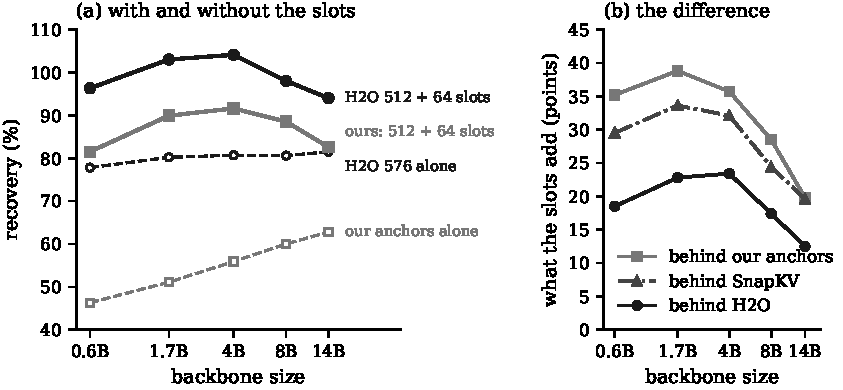
\includegraphics{fig_scale.pdf}
\caption{Table~\ref{tab:scale}'s lower block. (a) Solid lines add 64 learned
slots to a fixed selection; dashed lines spend the same budget without them.
(b) The difference between each pair, with SnapKV's selection added: what the
slots add rises to 1.7B--4B and then falls, behind all three selectors.}
\label{fig:scale}
\end{figure}

Figure~\ref{fig:scale} shows the shape. Each resource on its own is flat across
a 23-fold range of parameters: 576 learned slots recover $+53$ to $+60$
everywhere, 512 rarity-chosen verbatim entries $+21$ to $+30$, and 576 entries
chosen per head by H2O $+78$ to $+82$. What moves is what the learned state adds
behind a fixed selection. Behind our speculative anchors it rises from $+35.2$
at 0.6B to $+38.8$ at 1.7B and falls to $+19.8$ at 14B; behind H2O's selection
it rises from $+18.5$ to $+23.4$ at 4B and falls to $+12.5$. The same shape
appears behind SnapKV and in absolute nats, so it is an artefact neither of one
selector nor of the normalisation; the nats row is given because 14B's gap is
0.05 nats wider than the others'.

Our full method is the sum of this falling term and a rising one: the
speculative anchors on their own improve steadily with scale ($+46.3$ to
$+62.8$), since they are drafted from the state and read by a larger model. Its
recovery therefore peaks in the middle ($+91.6$ at 4B) and returns at 14B to
about where it started ($+82.6$ against $+81.5$ at 0.6B).

The two 8B runs differ in learning rate and seed. The first used the learning
rate tuned at 0.6B, whose training curve peaked around step 500 and then
declined---the signature of too large a step---and the checkpoint we must use is
the final one; the second, at $2.5\times$ lower learning rate, trained cleanly.
They differ by 3.6 points on the full method, because the anchors are drafted
from the state and so differ between runs, but by 1.8 points on what the state
adds behind them ($+28.5$ and $+30.3$), which is the quantity the argument rests
on.

What scales, then, is neither memory on its own but the marginal value of the
learned one. We do not have a mechanism, and the obvious candidate does not
survive contact with the data. The memory module's parameter count grows with
the backbone (3.7M to 26.2M) against a fixed training budget, so under-training
would predict the \emph{smallest} module to add the most---but 0.6B is not the
peak, which sits at 7--12M parameters with both ends lower. Something about the
middle of this range suits a 64-slot summary beside exact entries, and five
points do not say what.

One further observation, offered as a lead rather than an explanation:
randomly initialised slots are catastrophic at 0.6B ($-64.7\%$, against
$+46.3\%$ for no slots behind the same anchors) and nearly harmless at 14B
($+60.9\%$ against $+62.8\%$). Larger backbones tolerate arbitrary synthetic KV
entries that smaller ones cannot read. Whatever makes a large model forgiving of
noise in its cache may also make it less responsive to the structure a trained
compressor puts there.

\paragraph{Reading this result carefully.}
Two cautions, because the shape of this curve invites over-reading. First, each
scale point is a single training run apart from 8B; at 0.6B the seed spread is
1.8 points on the full method and 4.5 on what the state adds
(Table~\ref{tab:twobytwo}, at 8192 tokens), below the 19-point decline here but
an extrapolation to the larger points.
Second, and more important for anyone extending this: we obtained a clean
monotone increase from an earlier, pooled version of this comparison, in which
the 4B point came from a different machine, a different quantisation and a
different corpus than the others. Each individual correction was small---1.2
points for NF4, 0.3 for the corpus---and together they manufactured a trend that
the controlled sweep does not show. Small, individually defensible corrections
compose into artefacts.

\paragraph{The effective window is about one segment.}
A rolling state that has passed over all 8192 tokens recovers $+61.5\%$;
compressing \emph{only the most recent 512} recovers $+65.6\%$. Carrying the
state forward therefore dilutes rather than accumulates, and the distant past is
better served by anchors than by a longer chain of compression. Recurrent
compressive memories are known to concentrate on the recent past
\citep{compressive,lcirc}; the contribution here is that on this task the rolling
variant is not merely no better but worse than not rolling at all, which changes
what one should build.

\section{Two measurement hazards}
\label{sec:hazards}

\subsection{Fine-tuning the backbone deflates the denominator}

\begin{table}[ht]
\centering
\begin{tabular}{lcccc}
\toprule
 & \textsc{upper} & \textsc{lower} & gap & recovery \\
\midrule
backbone frozen & 3.459 & 3.951 & 0.492 & $\mathbf{+66\%}$ \\
LoRA enabled    & 3.037 & $\mathbf{3.370}$ & $\mathbf{0.332}$ & $+8\%$ \\
\bottomrule
\end{tabular}
\caption{Identical learning rate, identical step count; the only difference is
whether the backbone may adapt. The adapter improves ``predict the continuation
from nothing'' by 0.58 nats, removing a third of the denominator in
Eq.~\ref{eq:recovery}.}
\label{tab:lora}
\end{table}

The adapter is not learning to compress. It is doing language-model fine-tuning
on the evaluation distribution, and one side effect is that the task gets
easier. Note the direction of the trap: here it made the frozen number look
better, because the same slots were measured against an undeflated denominator.
In general the sign depends on which configuration is being promoted, which is
precisely why the confound is worth naming.

\paragraph{Scope.} This affects relative metrics of the form
Eq.~\ref{eq:recovery} only. Work reporting absolute downstream accuracy is
unaffected, and work that fine-tunes both a compressor and a reader for
deployment is doing something legitimate that this critique does not touch. See
\S\ref{sec:related} for the closest prior statements.

\subsection{Variance is largest where the headline is}

\begin{table}[ht]
\centering
\begin{tabular}{lccccr}
\toprule
configuration & seed 0 & seed 1 & seed 2 & & spread \\
\midrule
16 slots ($32{:}1$) & $+15$ & $+41$ & $+66$ & & \textbf{51 points} \\
32 slots ($16{:}1$) & $+105$ & $+66$ & $+103$ & & \textbf{39 points} \\
72 slots & $+114$ & $+109$ & $+111$ & & 5 points \\
128 slots & $+115$ & $+111$ & $+112$ & & 4 points \\
\midrule
hybrid, six conditions (\S\ref{sec:decomposition}) & & & & & 1.6--4.8 points \\
\bottomrule
\end{tabular}
\caption{Identical data and hyperparameters; only the random seed differs. The
first four rows are single-hop recovery measured during training, which is why
they exceed $100\%$ and are not comparable to the multi-hop figures elsewhere;
what matters is the spread down each row. The last row covers the six cells of
Table~\ref{tab:twobytwo}, excluding the randomly initialised state, whose slots
are re-drawn per window and unseeded by construction.}
\label{tab:variance}
\end{table}

The compression ratios that are most attractive to report are the ones whose
results are least reproducible. We found this the hard way: a checkpoint was
lost and retrained under identical settings, and the 16-slot figure moved from
$+83\%$ to $+38\%$. Any claim in this area resting on a few points---including
several we had provisionally drawn about scale---requires its own spread before
it means anything. We recommend reporting seed spread at the highest compression
ratio claimed, and we note that the hybrid architecture is not merely better on
average but an order of magnitude more stable, which may be the more important
property.

\section{Related work}
\label{sec:related}

Our instrument is assembled from published components; what follows separates
what we borrowed from what we are claiming.

\paragraph{Discarding or approximating real cache entries.}
One family keeps the cache made of real entries and decides which to drop.
\citet{h2o} retain a recent window plus persistent heavy hitters identified by
accumulated attention; \citet{snapkv} select using an observation window at the
end of the prompt; \citet{pyramidkv} allocate unequal budgets across depth.
\citet{streamingllm} show that the first few positions act as an attention sink
whose removal is catastrophic---a result we depend on operationally, since every
partial-cache condition in this paper would otherwise collapse.
\citet{kivi} approximate rather than evict, quantising the cache to two bits.
\citet{quest} and \citet{infllm} keep the full cache but attend sparsely, scoring
blocks or representative tokens to decide what to load; Quest in particular
selects per attention head from the current query, which is the granularity our
own retrieval lacks (\S\ref{sec:baselines}). These methods never fabricate
entries, so the distribution constraint we report in
\S\ref{sec:decomposition}---that untrained synthetic slots are worse than no
slots---does not arise for them. We compare against three of them at a matched
budget, alone and with our slots behind them, in \S\ref{sec:baselines}.

\paragraph{Learning to compress context into slots.}
The second family replaces spans of context with a small number of learned
vectors: gist tokens \citep{gist}, autoencoding into memory slots \citep{icae},
summary vectors trained by continued adaptation \citep{autocompressor}, and
aggressive prompt compression \citep{500x}. Recurrent variants compress
repeatedly as the sequence advances \citep{compressive,rmt,lcirc}. Our compressor
is a minimal member of this family---learned slot embeddings plus a per-layer
bias at memory positions in the manner of prefix tuning \citep{ptuningv2}---and we
make no claim for it. We hold the backbone frozen throughout, which within this
family is closest to \citet{icae}, \citet{arcencoder} and \citet{500x}.

\paragraph{Pairing compressed memory with exact entries.}
The hybrid we measure has been proposed. \citet{strongdrafts} combine compressed
distant slots with exact recent entries for speculative decoding, discarding the
distant verbatim cache rather than retrieving it. \citet{specache} keep verbatim
KV on the CPU and prefetch it by predicting what the next step will attend to,
which is the speculative-retrieval mechanism we use as our deployable policy. At
the agent-memory level, \citet{justmem} and \citet{infinimemory} both contrast
reading a compressed representation against fetching the source, and both find
neither alone suffices---consistent with our decomposition, though at the level
of task accuracy with retrieval set and summariser varying together, rather than
holding one fixed to attribute the difference. We treat all four as prior art for
the architecture and confine our claims to the attribution.

\paragraph{Whether to freeze the reader.}
Freezing is usually motivated by plug-and-play reuse or by preserving abilities
outside the compression task \citep{icae,arcencoder,500x}; \citet{cocom} argue the
opposite for retrieval-augmented generation, holding that a frozen decoder cannot
make good use of compressed context, and \citet{spkv} continue pretraining the
model jointly with their utility predictor. Closest to \S\ref{sec:hazards},
\citet{ccm} report that naively fine-tuning the whole model during compression
training lets it answer without consulting the memory at all---their no-context
training loss falls from 2.69 to 1.84 while test loss stays at 2.59---and freeze
the LM in response. They frame this as overfitting on inputs, i.e.\ a training
pathology. \citet{simplecc} adopt a normalisation nearly identical to
Eq.~\ref{eq:recovery} in order to discount questions answerable without context,
but fine-tune adapters on both sides and present the correction as a property of
the question set. Our addition is narrow: the same effect read as an
\emph{evaluation} confound, with a magnitude attached (0.58 nats, a third of the
denominator) and a stated scope. We do not claim the principle is new.

\paragraph{Compressibility depends on the task.}
That compression costs vary sharply across task types is established
\citep{kvbench,shotkv}. Our dialogue-versus-prose gap figures (1.269 against 0.286
nats) are reported in that spirit---as a caution about which corpora can support
this measurement at all---and not as a finding.

\paragraph{Per-token analyses of long context.}
Nearest to \S\ref{sec:copyability}, \citet{tokensbenefit} stratify token-level
perplexity by how often an $n$-gram occurs in the added context and find that
newly appearing material correlates with the benefit from a longer window, but
they study \emph{uncompressed} long-context models, so the question of what
compression specifically destroys does not arise. \citet{gistboundary} analyse
gist-based compression at finer grain than task accuracy and find unexpected
information is lost preferentially---topically relevant word needles at 50.7
against surprising ones at 35.8 under $8\times$ compression---which points the
same direction as our result while grouping by a needle's relation to the topic
rather than by whether the target token was copyable. To our knowledge the
grouping we use, over the tokens actually being predicted under compression, has
not been reported; \S\ref{sec:limitations} states the limits of that claim.

\section{Limitations}
\label{sec:limitations}

\begin{itemize}
\item \textbf{Mostly perplexity, and one synthetic task.} Apart from
\S\ref{sec:needle} every number here is token cross-entropy on held-out
continuations. The needle task is synthetic and of our own construction; it
establishes the endpoint of the copyability axis rather than performance on
anything anyone wants done. Established suites---LongBench, RULER---would test
whether the two regimes we describe appear at the mix of copyable and inferable
answers that real tasks have, and we do not run them.
\item \textbf{One model family, five scale points, one repeated.} Qwen3 at
0.6B, 1.7B, 4B, 8B and 14B in a single matched sweep, with 8B repeated at a
second learning rate. The seed spread underpinning the comparison was measured
at 0.6B and extrapolated upward, and every point except 8B is a single run.
Larger dense points would show where the decline ends; MoE backbones would test
whether it is specific to dense models, but that introduces an architecture
difference this sweep deliberately avoids.
All five points were trained in bf16 with the same corpus and settings (14B on
a second, larger rented card) and re-evaluated for this version on a single
card; an earlier, pooled version of this comparison mixed NF4 and a
different corpus, and \S\ref{para:scale} describes what that did.
\item \textbf{An instability we could not pin down.} In an earlier 1.7B
configuration the rolling state diverged under multi-hop recursion---$-101.5\%$
and $-47.3\%$ on two seeds---while single-segment states from the same
checkpoints behaved normally. The 1.7B point in the controlled sweep
(Table~\ref{tab:scale}) shows no such divergence ($+53.2\%$ on the same
condition), so whatever causes it is not the scale point itself; the runs differ
in corpus, host and PyTorch version, and we did not isolate which. We mention it
because anyone reproducing the rolling conditions may encounter it, and because
it is the reason we report the sweep from single-segment states.
\item \textbf{Our retrieval is the weak component.} It selects one set of
positions for every layer from last-layer attention, and per-head selection beats
it on both tasks: H2O's selection with our slots behind it recovers $+101\%$
against our $+88.6\%$ on text, and SnapKV answers $99\%$ of needles against our
$12\%$ given the same question (\S\ref{sec:baselines}). We did not rebuild the
method around per-head retrieval; anyone using this architecture should.
\item \textbf{The baseline comparison is not like-for-like.}
\S\ref{sec:baselines} matches memory budget, not training cost: H2O, SnapKV and
StreamingLLM require no training step and no corpus, while our module is trained
on the evaluation domain and is domain-specific. The table says what a small
learned component buys at a fixed budget; it does not say those policies are
badly designed, and a deployment that cannot train on its own traffic is one
where they win by default. Our H2O and SnapKV are reimplementations from their
papers' descriptions, not the reference code, and reference implementations
differ in details such as pooling and per-layer budgets.
\item \textbf{Corpus.} The dialogue corpus is a private collection of real
conversation logs and cannot be released. Gap figures for a public prose corpus
are given for contrast, and the low gap there ($0.286$ nats) is itself a warning
about which corpora can support this kind of measurement.
\item \textbf{The literature search is not exhaustive.} Our ``to our knowledge''
claims rest on a bounded survey: a written brief stating the two questions and
the finding we expected to be pre-empted was given to a search-capable model,
whose returned claims were then re-checked, and every arXiv identifier cited here
was subsequently resolved against the arXiv API to confirm that the paper exists
and that its title and first author match. That procedure establishes what we
read, not what exists; several of our conclusions did turn out to be
pre-empted and are cited as such in \S\ref{sec:related}. We phrase the remaining
two as ``to our knowledge'' rather than as priority claims, and would rather be
corrected on them than defend them.
\end{itemize}

\section*{Changes from version 1}

Version 1 (\href{https://doi.org/10.5281/zenodo.22897854}{10.5281/zenodo.22897854})
contained a bug and several errors, corrected here.

\paragraph{The bug.} Every policy that selects context by attention---our
deployable retrieval and our implementations of H2O and SnapKV---recomputes
attention by hand, since the fused kernel does not return weights. Version 1 did
so without applying the rotary position embedding to the query, while the cached
keys carry it. The scores were therefore not the model's attention: on a test
sequence their top 32 positions agreed with the model's own on one. This version
rotates the query and checks the hand-computed attention against the eager
implementation at every layer before any experiment runs. Oracle selection, which
matches tokens rather than scoring attention, and every result that involves no
retrieval---the copyability decomposition, the abstract-state figures, the
fine-tuning confound---were unaffected and are unchanged.

\paragraph{What changed as a result.}
\begin{itemize}
\item \textbf{Baselines.} H2O and SnapKV now select per layer and per KV head, as
specified; version 1 applied one set of positions from the last layer to every
layer and ran SnapKV's observation window without its preceding context. Version
1's comparison ($+89.5\%$ against a best baseline of $+55.8\%$) is replaced by
Table~\ref{tab:baselines}: $+88.6\%$ against H2O's $+77.9\%$, and H2O's selection
with our slots behind it at $+101.1\%$.
\item \textbf{The needle comparison.} Version 1 reported that our method placed
last on the needle task because its query was a drafted guess. That was wrong
independently of the bug: on the needle task our retrieval already used the
question, and our SnapKV never saw it. With correct scoring the outcome is
decided by whether the selector sees the question and selects per head
(Table~\ref{tab:inversion}); version 1's Figure 2 is withdrawn.
\item \textbf{Decomposition.} The deployable row of Table~\ref{tab:twobytwo}
moves from $+31.4$, $+71.9$, $+75.4$ to $+32.6$, $+74.7$, $+77.8$; the oracle row is
unchanged and so are the conclusions.
\item \textbf{Anchor budget.} The checkpoint behind version 1's
$+87.8\to+96.6$ row no longer exists; the row is remeasured with the three
checkpoints used elsewhere.
\item \textbf{Scale.} The sweep was re-evaluated on one card. The full
method's row moves from $+82.6$, $+90.2$, $+90.1$, $+83.3$, $+75.9$ to $+81.5$,
$+89.9$, $+91.6$, $+88.5$, $+82.6$: the peak stays at 1.7B--4B, but 14B no longer
falls below 0.6B. Rows that involve no attention scoring reproduce version 1 to
within 0.2 points on the new card. Version 1 also measured the hybrid's gain against anchors
chosen by rarity rather than against its own anchors; Table~\ref{tab:scale} now
reports what the state adds behind the same entries, which peaks at 1.7B--4B and
roughly halves by 14B behind three selectors. Version 1's statement that the two
8B runs agree within a point holds for that quantity (1.8 points) but not for
the full method (3.6).
\item \textbf{Mislabels.} The oracle row of version 1's needle table read ``512
anchors''; it used the needle's own 16 tokens and the 4-token sink, beside the 64
slots. The limitations text still described an earlier plan (4B under NF4, 8B
missing) that the controlled sweep had already superseded.
\end{itemize}

\section*{Use of AI assistance}

All experiments, analysis, debugging (including identifying the attention-scoring
bug that necessitated version 2) and scientific conclusions in this paper are the
author's own work. An AI writing assistant (Anthropic's Claude) was used to help
draft and edit the English prose. The author reviewed and takes responsibility
for the final text.

\section*{Reproducibility}

Code, logs and the full experimental record---including the intermediate
conclusions that were later falsified---are at
\url{https://github.com/HoshiGT/frozen-kv-memory}. The dialogue corpus is
withheld for privacy reasons; the prose corpus and its preparation script are
included.

\bibliographystyle{plainnat}
\bibliography{refs}

\end{document}
